\documentclass{article}

\usepackage[a4paper, total={6.5in, 11in}]{geometry}
\usepackage{graphicx}
\graphicspath{{titech/CSC.T527.FaultTolerantDistributedAlgorithm/}}

\usepackage{latex/common}

\title{FTDA 2021 - Homework 3}
\author{Sixue Wang\\Tokyo Institute of Technology}

\begin{document}

\maketitle

\section*{Question 1}
I will explain why a protocol that works in 3 processes cannot work in multiple crashes. The essential point is that majority of processes don't make a consensus of ``learn'' messages(ready to deal with the same message).

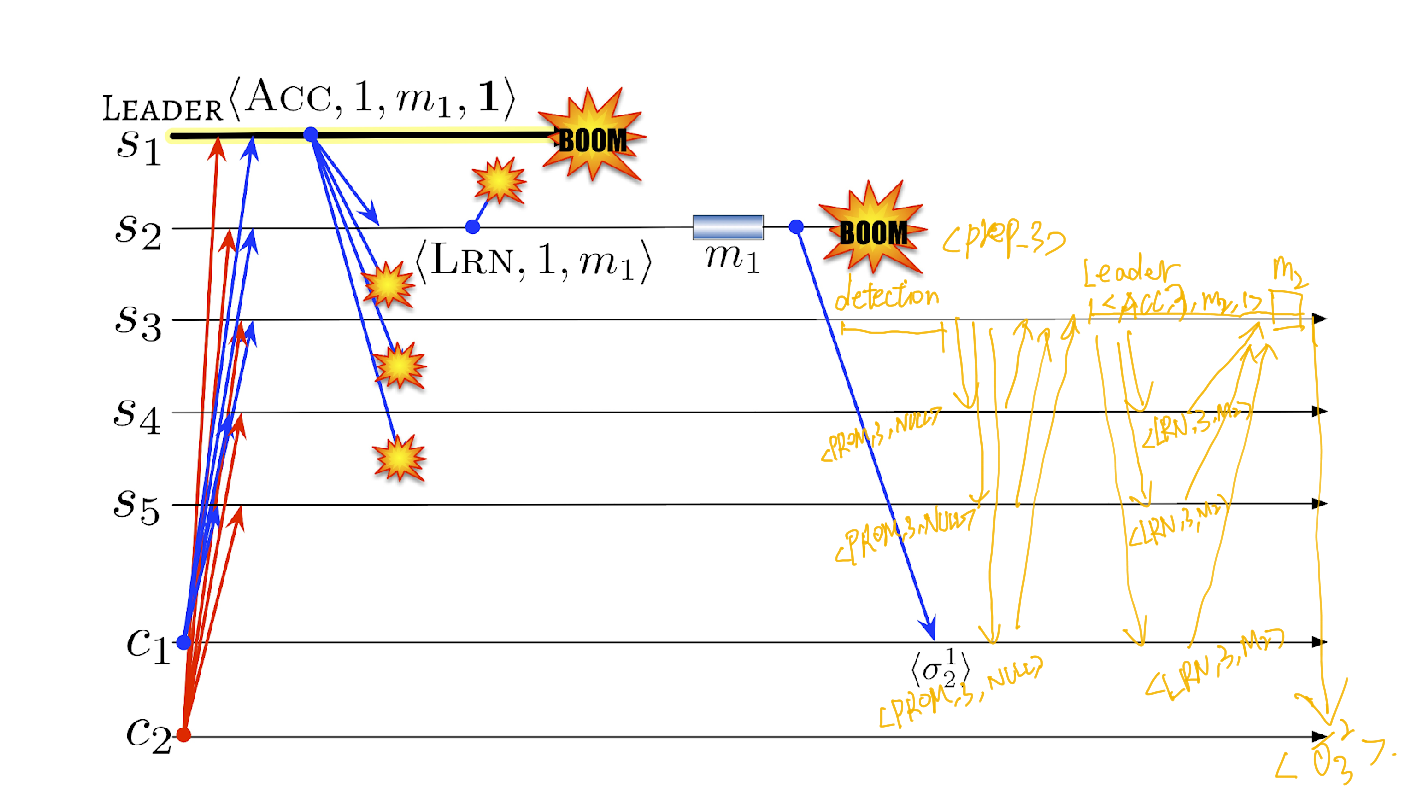
\includegraphics[width=\textwidth]{hw3_1}

\section*{Question 2}
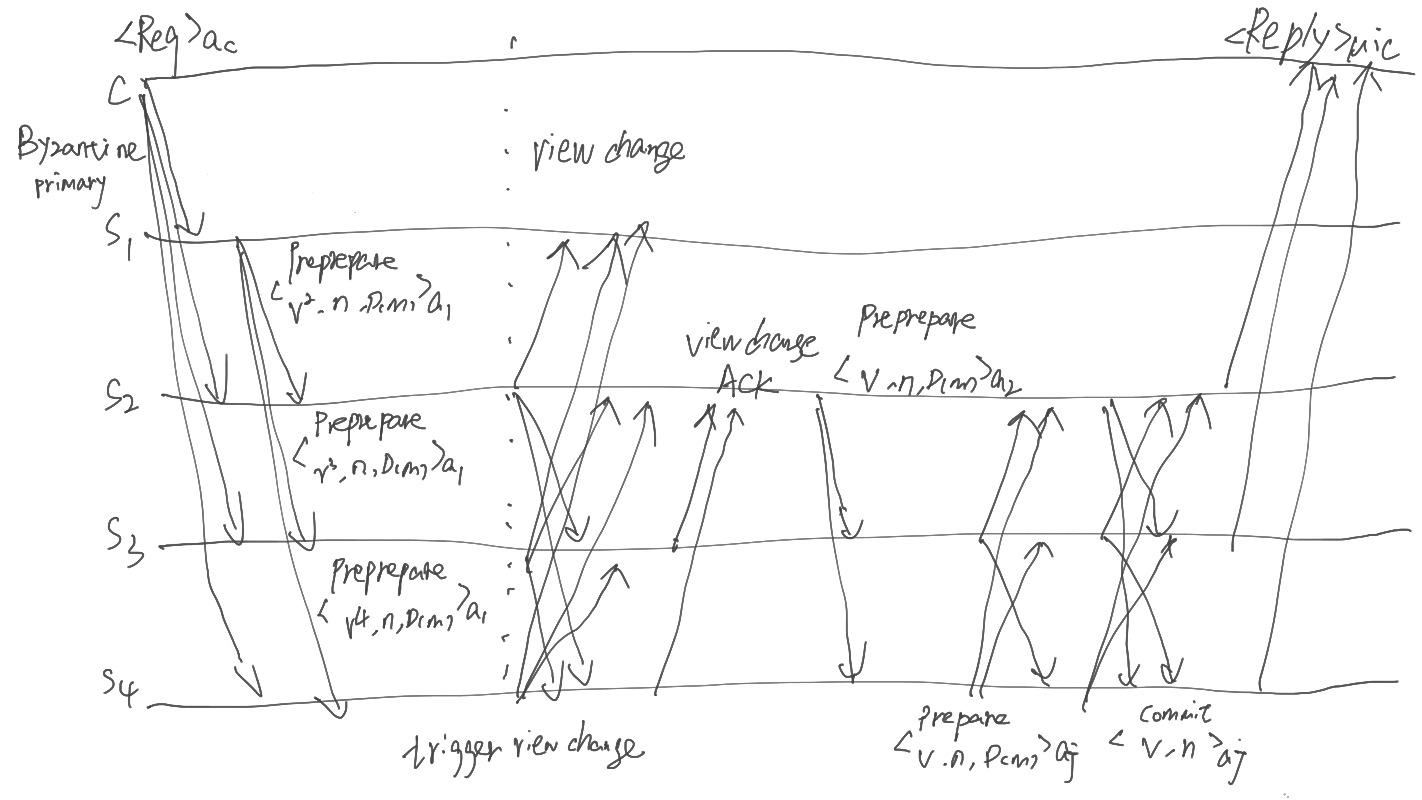
\includegraphics[width=\textwidth]{hw3_2}
In my setting, there are 1 cilent and 4 servers and $s_1$ is a Byzantine primary. The execution is described as follows:
\begin{enumerate}
  \item Request: Client sends the ``Resquest'' to all servers. Every server must have the original resquest to get the hash value.
  \item Preprepare: The primary sends ``Preprepare'' to other servers just like ``ACC'' in Paxos. In my example, the primary sends different view numbers to different servers. Actually the Byzantine primary can do other faulty action.
  \item Trigger View-change: At that time, backup servers can detect that the primary is a Byzantine server. Personally, I think one server will exchange suspicion with other backup servers when it found something wrong. If majority of backup servers have consensus of that, then they will trigger view-change.
  \item View-change: Backup servers send ``ViewChange'' to all other servers, then wait for ``ViewChangeACK''. Now $s_2$ is the primary.
  \item Preprepare: The primary $s_2$ sends ``Preprepare'' to other servers.
  \item Prepare: Backup servers exchange ``Prepare'' with other backup servers to certificate.
  \item Commit: $s_{2-4}$ have the consensus of ``Prepare'' so they process the request and commit to each other.
  \item Reply: All committed servers send ``Reply'' to the client.
\end{enumerate}



\section*{Question 3}
For a round-synchronous model, we can always detect which processes crashed, so $n$ is determined by $f_B$, and I think the round-synchronous model could not improve the lower bound, so $n \geq 3f_B+1$.

On the other hand, the lower bound of the number of round is different. We need $f_C$ rounds at least to detect all crashed processes and need more $f_B$ rounds to deal with unreplied Byzantine processes. After this, we still need $f_B+1$ rounds to solve Byzantine lies, so we need $f_C+2F_B+1$ rounds totally.

To be honest, I'm not 100\% sure why unreplied Byzantine and Byzantine lies would have no intersection not only in my answer but also in the lecture. I mean if we can detect some Byzantine processes don't reply, then we could kick them off our cluster so they have no opportunity to lie. One possible way is that the Byzantine process disguis as another process and does not reply. But I have no idea how could do that.

\end{document}
